\vspace*{6cm}
{\setlength{\parskip}{-0.5cm}
\chapter{Marco Metodológico}
}

\newpage

En este capítulo se establecen el tipo y nivel de investigación, la población y muestra, los instrumentos de recolección de datos, el procedimiento, las técnicas de análisis de datos y el cronograma de actividades detalladas en los objetivos del proyecto.

{\setlength{\parskip}{0cm}
\section{Descripción del área de estudio}

El área de estudio total consistió en la Urbanización Guaraguao Campo Obrero, de superficie aproximada de 387.800 m$^2$ y ubicada en Puerto La Cruz, estado Anzoátegui. Del área total, el estudio del proyecto se enfocó en la calle 11 de la urbanización. La zona se encuentra delimitada por el borde rojo mostrado en la figura 3.1, donde además se muestran el conjunto de calles y avenidas de la zona.
}

\begin{figure}[h]
    \centering
    \captionsetup{singlelinecheck=false, justification=raggedright, labelsep=newline}
    \caption{\textit{Mapa satelital de la Urbanización Guaraguao de Puerto La Cruz}}
    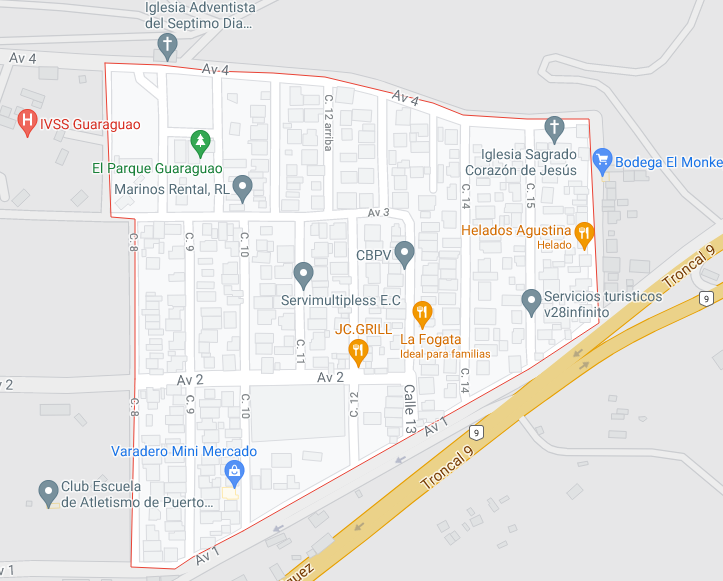
\includegraphics[width=15cm]{Media/Urb Guaraguao.png}
    \raggedright Fuente: Google Maps
    \label{fig:mapa}
\end{figure}

{\setlength{\parskip}{0cm}
\section{Nivel de Investigación}

\say{El nivel de investigación se refiere al grado de profundidad con que se aborda un fenómeno u objeto de estudio. Según el nivel, la investigación se clasifica en: Investigación Exploratoria, Investigación Descriptiva e Investigación Explicativa} (Arias, 2012).
}

En este proyecto de investigación se manifestó un nivel de investigación descriptivo. \say{La investigación descriptiva consiste en la caracterización de un hecho, fenómeno, individuo o grupo, con el fin de establecer su estructura o comportamiento.} (Arias, 2012). Se encuentra en dicho nivel, debido a que se caracterizaron las técnicas de manejo de los desechos sólidos de la población de la Urbanización Guaraguao Campo Obrero, y también, se estudiaron los beneficios de las 3R de la ecología y su aplicación en el área de estudio. 

{\setlength{\parskip}{0cm}
\section{Tipo de Investigación}

\say{El tipo de investigación es la estrategia general que adopta el investigador para responder al problema planteado. En atención al tipo, la investigación se clasifica en Investigación Documental, Investigación de Campo e Investigación Experimental.} (Arias, 2012).
}

El tipo de investigación que correspondió a este proyecto de investigación fue de campo. \say{La investigación de campo es aquella que consiste en la recolección de datos directamente de los sujetos investigados, o de la realidad donde ocurren los hechos (datos primarios).} (Arias, 2012). Es de campo porque se recolectaron los datos directamente de la población de la Urbanización Guaraguao de Puerto La Cruz, aplicando las técnicas e instrumentos propuestos para cumplir con los objetivos planteados.

{\setlength{\parskip}{0cm}
\section{Población y muestra}

\subsection{Población}

\say{La población, o en términos más precisos población objetivo, es un conjunto finito o infinito de elementos con características comunes para los cuales serán extensivas las conclusiones de la investigación. Ésta queda delimitada por el problema y por los objetivos del estudio.} (Arias, 2012). En este estudio, la población fue finita y consistió en, aproximadamente, 700 casas de la Urbanización Guaraguao de Puerto La Cruz.
}

{\setlength{\parskip}{0cm}
\subsection{Muestra}

\say{La muestra es un subconjunto representativo y finito que se extrae de la población accesible} (Arias, 2012). La muestra representativa estuvo compuesta por 22 casas pertenecientes a la calle 11 de la Urbanización Guaraguao Campo Obrero. Dicha muestra fue seleccionada mediante el muestreo intencional u opinático \say{En este caso los elementos son escogidos con base en criterios o juicios preestablecidos por el investigador.} (Arias, 2012).
}

{\setlength{\parskip}{0cm}

\section{Técnicas e Instrumentos de Recolección de Datos}

\say{Las técnicas de recolección de datos son procedimientos o fórmulas particulares de obtener datos o información}. (Arias, 2012).
}

\say{Un instrumento de recolección de datos es cualquier recurso, dispositivo o formato (en papel o digital), que se utiliza para obtener, registrar o almacenar información}. (Arias, 2012).

En este proyecto de investigación se emplearon las siguientes técnicas e instrumentos de recolección de datos:

\begin{itemize}
    \item Se utilizó la encuesta escrita como técnica de recolección de datos: “Se define a la encuesta como una técnica que pretende obtener información que suministra un grupo o muestra de sujetos acerca de sí mismos, o en relación con un tema particular. La  encuesta puede ser oral o escrita. La encuesta escrita es la que se realiza mediante un cuestionario” (Arias, 2012). Su instrumento correspondiente fue el cuestionario de preguntas cerradas: “El cuestionario es la modalidad de encuesta que se realiza de forma escrita, está formado por una serie de preguntas. El cuestionario puede ser de preguntas cerradas (cuando se establecen previamente las posibles respuestas), abiertas (cuando no ofrecen opciones de respuesta) y mixtas (cuando combina preguntas abiertas y cerradas)” (Arias, 2012). Fueron empleados con el fin de determinar los hábitos del manejo de desechos sólidos de la muestra y evaluar el conocimiento que poseían respecto a este tema a través de preguntas cerradas.
    
    \item Se usó la observación estructurada participante como técnica de recolección de datos: “La observación es una técnica que consiste en visualizar o captar mediante la vista, en forma sistemática, cualquier hecho, fenómeno o situación que se produzca en la naturaleza o en la sociedad. La observación participante es cuando el investigador pasa a formar parte de la comunidad o medio donde se desarrolla el estudio, se clasifica en observación no estructurada y observación estructurada. La observación participante estructurada es aquella que además de realizarse en correspondencia con unos objetivos, utiliza una guía diseñada previamente, en la que se especifican los elementos que serán observados” (Arias, 2012). Su instrumento correspondiente fue la lista de cotejo, “Es un instrumento en el que se indica la presencia o ausencia de un aspecto o conducta a ser observada.” (Arias, 2012), y la lista de frecuencia \say{Es un instrumento que se diseña para registrar cada vez que se presenta una conducta o comportamiento} (Arias, 2012). Fueron utilizados para la recolección de datos ya que permitían registrar de forma organizada la frecuencia con que se aplicaron las estrategias propuestas para poner en práctica las 3R de la ecología en la muestra seleccionada.
\end{itemize}

{\setlength{\parskip}{0cm}
\section{Procedimiento}

En primer lugar, se describieron los beneficios que traen consigo la aplicación de las 3R de la ecología. Para ello, se realizó una investigación documental sobre los mismos explicando el porqué es importante implementar los métodos de reciclaje, reducción y reutilización en la vida cotidiana de las personas, y los beneficios que acarrea esto para las comunidades y el medio ambiente.
}

Después, se determinaron los métodos empleados por la población para el manejo adecuado de la basura. Los habitantes del área de estudio explicaron sus hábitos para el manejo de desechos sólidos: si clasificaban una parte de los mismos, los materiales que reutilizaban para beneficio ambiental y propio, etc. 

Para ello, se aplicó una encuesta escrita de 8 preguntas cerradas a los 22 hogares que representaron a la muestra seleccionada, y así conocer su rutina en el marco del manejo de basura.

Posteriormente, se realizó una campaña divulgativa sobre el manejo adecuado de los desechos sólidos para la sensibilización del uso de las 3R de la ecología, con el fin de que los habitantes de la urbanización tengan el conocimiento necesario acerca de las 3R (reducir, reciclar y reutilizar) y cómo ponerlas en práctica. En este paso se distribuyeron folletos por cada casa en la muestra seleccionada y se dio una breve charla explicando los beneficios de las 3R de la ecología en la comunidad y cómo a través de estrategias pueden poner en práctica sus principios en el ámbito doméstico. Además, se ejecutó una segunda encuesta escrita de 6 preguntas cerradas para determinar el impacto de la campaña divulgativa en los habitantes.

Finalmente, se efectuó un seguimiento de las estrategias propuestas para el empleo de las 3R de la ecología, observando que medidas planteadas en la campaña divulgativa se lograron poner en práctica por los habitantes y con que frecuencia. Para esto, se realizó la observación participante estructurada y se rellenaron listas de cotejo por cada hogar de la muestra seleccionada. 

{\setlength{\parskip}{0cm}
\section{Técnicas de Análisis de Datos}

\say{La aplicación sistemática de técnicas estadísticas y lógicas para describir el alcance de los datos, modular la estructura de los datos, condensar la representación de los datos, ilustrarlos mediante imágenes, tablas y gráficos, y evaluar las inclinaciones estadísticas, los datos de probabilidad, para obtener conclusiones significativas, se conoce como análisis de datos.} (Arteaga, 2020). Pueden provenir de varias fuentes y pueden tener formato de texto, de audio, de imagen o de vídeo.
}

Para analizar los resultados cuantitativos, se utilizaron las siguientes técnicas de análisis:

\begin{itemize}
    \item Gráfico de barras: \say{Un gráfico de barras es una forma de resumir un conjunto de datos por categorías. Muestra los datos usando varias barras de la misma anchura, cada una de las cuales representa una categoría concreta.} (TIBCO, 2014). Se empleó el gráfico de barras porque permitía comparar gráficamente cuales indicadores de las tablas presentaron mayor frecuencia en la población de estudio.

    \item Tabla: \say{En computación, una tabla hace referencia al modelado o recopilación de datos por parte de una aplicación de un programa que permite operar con los mismos organizándolos y poniéndolos en relación de diversas maneras. Son estructuras útiles y a menudo fáciles de interpretar para relacionar datos e información de manera pertinente.} (Bembibre, 2009). Se usó la tabla para poder recopilar de manera organizada los resultados cuantitativos que fueron obtenidos.
\end{itemize}

\newpage

\section{Cronograma} 

\begin{figure}[h]
    \centering
    \captionsetup{singlelinecheck=false, justification=raggedright, labelsep=newline}
    \caption{\textit{Cronograma de actividades detalladas en los objetivos del proyecto}}
    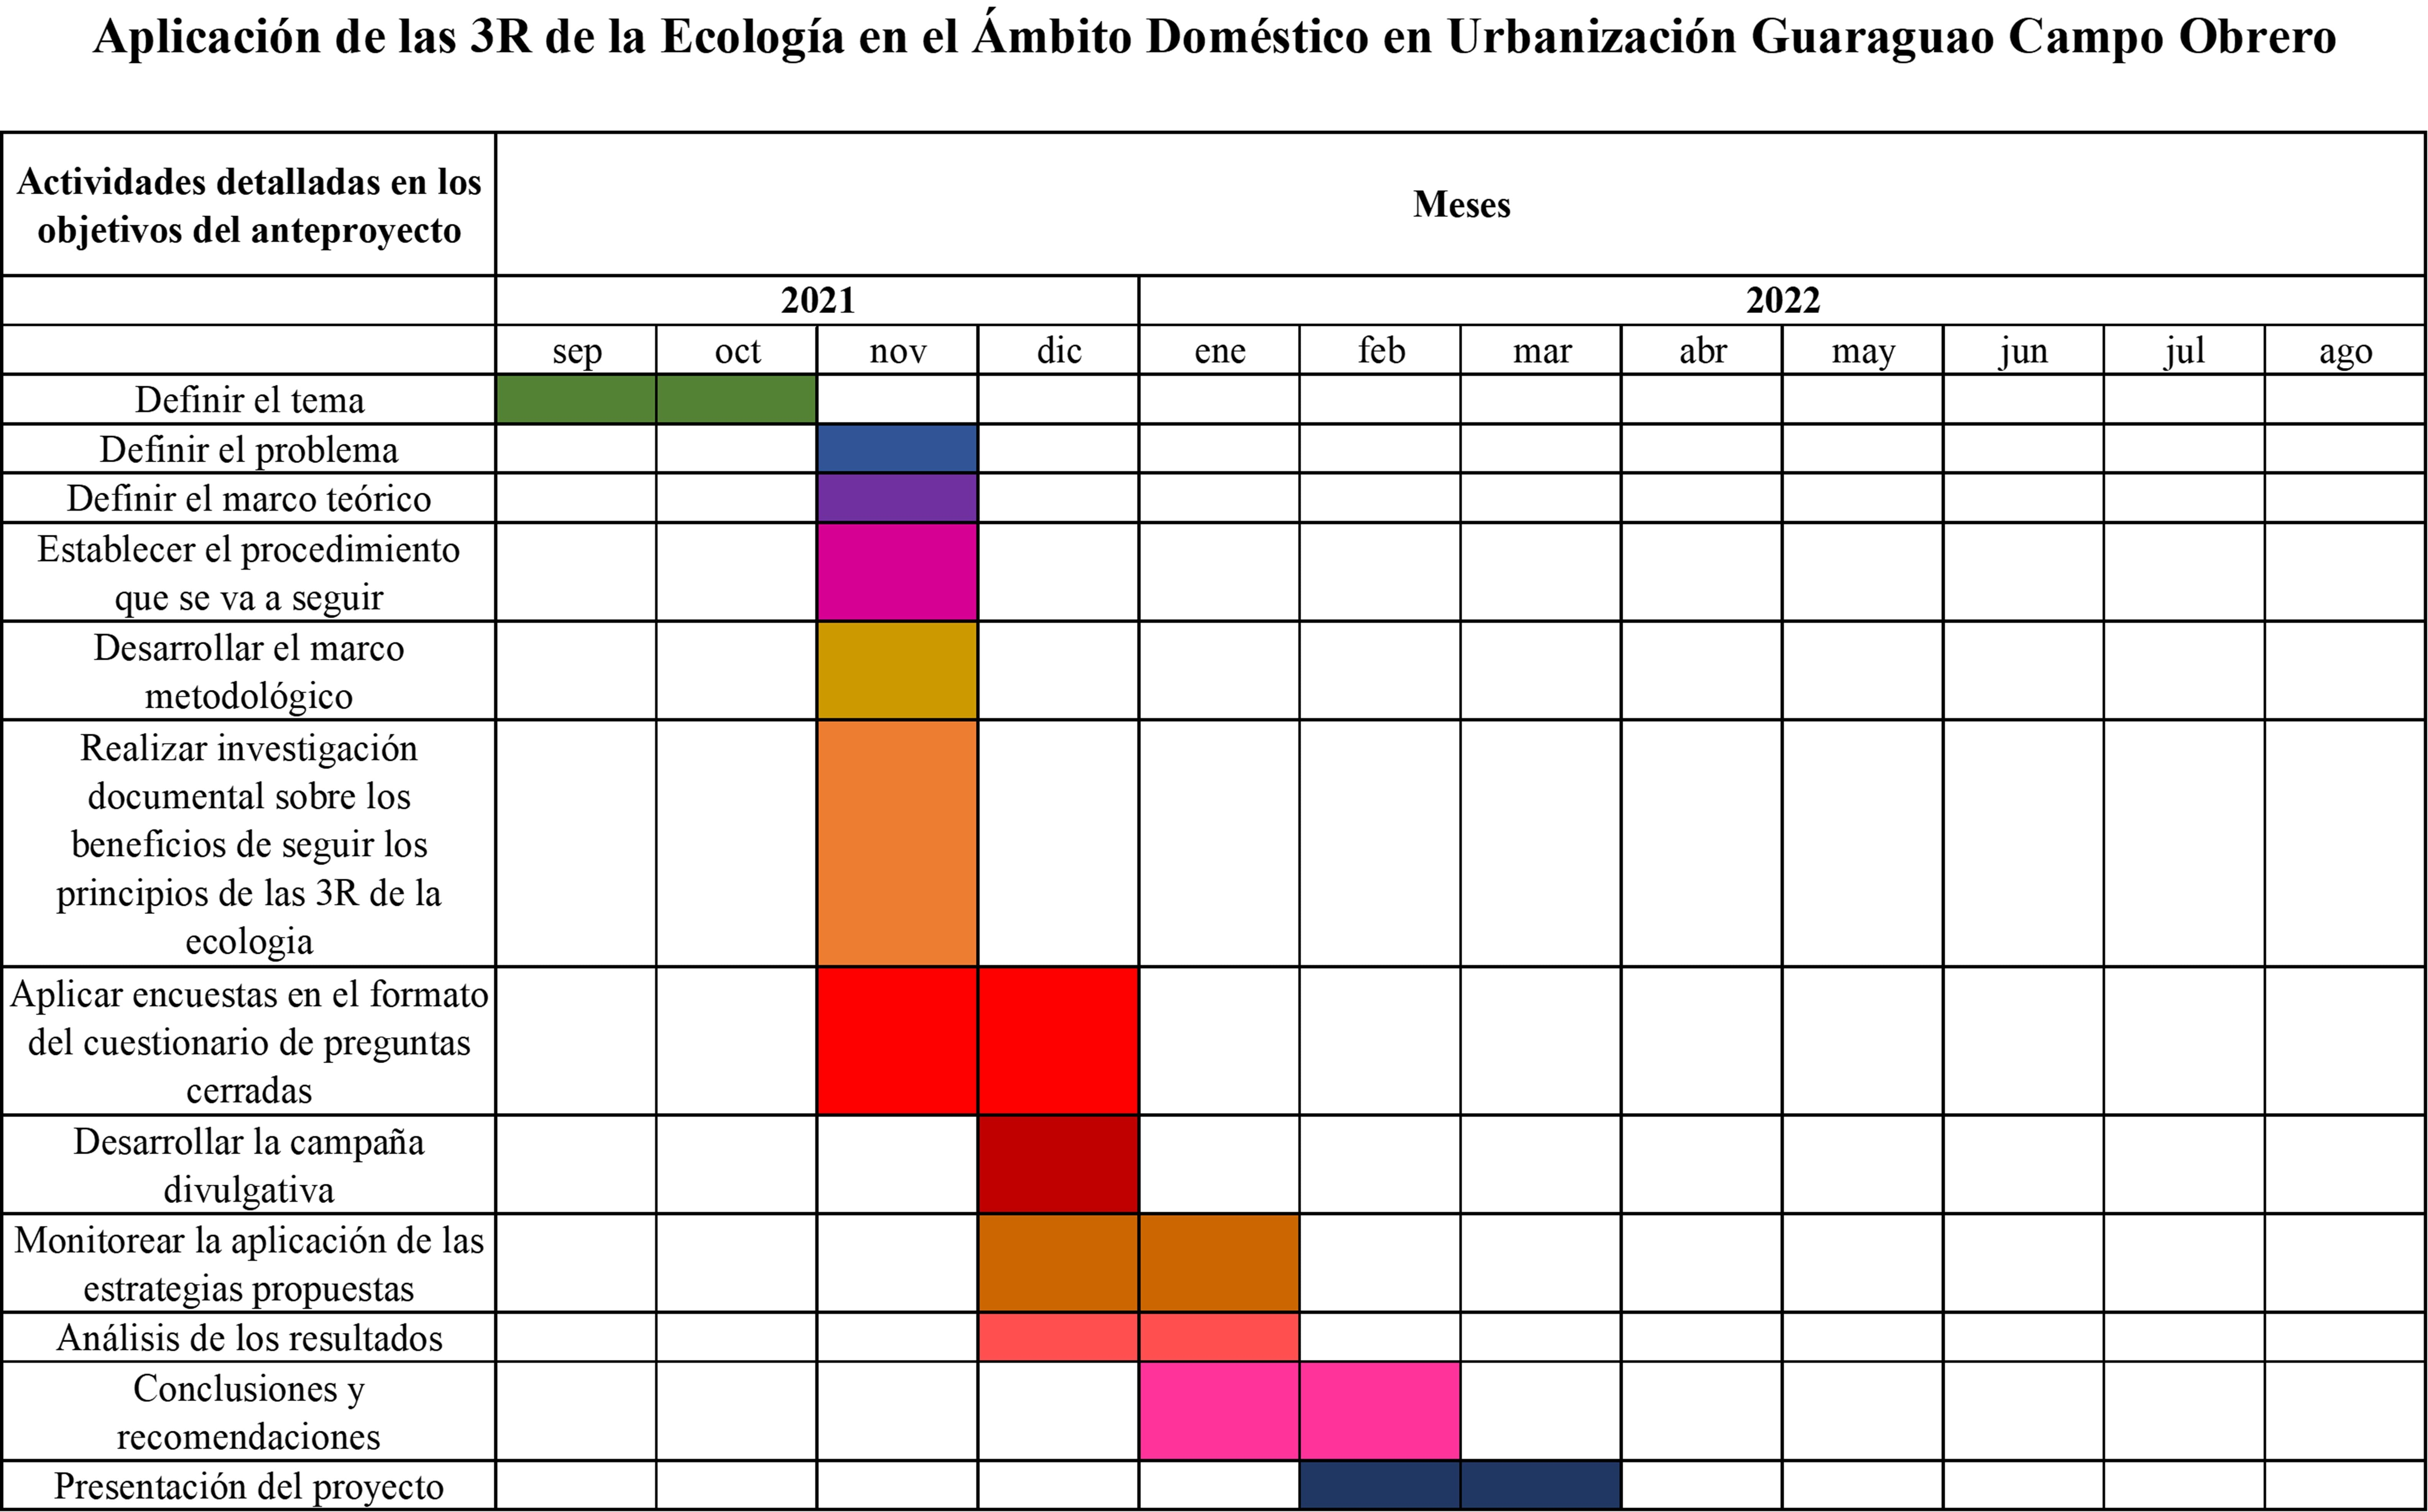
\includegraphics[width=15cm]{Media/Cronograma.jpg}
    \raggedright Fuente: Elaboración propia
    \label{fig:cronograma}
\end{figure}

\newpage